\chapter{Choix de développement}

\section{Les métadonnées}
\subsection{Utilisation des métadonnées stockées sur le disque dans le code
source de GELI}
\label{ssec:md_usage}
L'analyse de \textit{LUKS} et \textit{GELI} nous a montré les similitudes et
différences que présentent ces deux systèmes.
\paragraph{}
\begin{figure}[h]
\centering
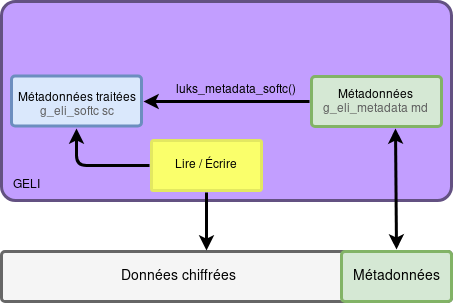
\includegraphics[width=.6\linewidth]{choix_developpement/utilisation_metadonnee.png}
\caption{\label{fig:softc_eli}Métadonnées en mémoire}
\end{figure}

\paragraph{}
Pour n'importe-quel module noyau utilisant la classe \textit{GEOM} de
\textit{FreeBSD}, les métadonnées sont toujours placées à la fin des données du
disque, contrairement à \textit{LUKS}. Il faut donc créer les fonctions
utilisant celles fournies par \textit{GEOM} afin de réaliser cette opération.
\paragraph{}
Dans le cas d'un fichier (utile pour sauvegarder l'en-tête contenant les 
métadonnées), il suffit d'utiliser les fonctions standards de
\verb|C| et de lire le début du fichier. Dans le cas d'un disque en revanche, il
faut créer une fonction lisant les premiers secteurs. On peut ensuite les
stocker dans une structure afin de connaître les propriétés de chiffrement
utilisées.

\paragraph{}
Les informations présentes dans les métadonnées \textit{LUKS} sont assez proches
de celles de \textit{GELI}:
\begin{itemize}
\item le \textit{MAGIC}
\item la version utilisée
\item l'algorithme de chiffrement
\item l'algorithme de hashage
\item le sel
\item le nombre d'itérations PKCS
\item la \textit{masterkey} chiffrée
\end{itemize}

\paragraph{}
Les métadonnées sont donc stockées sur le disque et sont mappées en mémoire via
la structure {\em md} de type {\em g\_eli\_metadata}. Mais des métadonnées 
"indirectes" sont aussi présentes en mémoire à travers la structure {\em softc} 
de type {\em g\_eli\_softc}. Comme illustré par le schéma \ref{fig:softc_eli} 
cette structure diffère des 
métadonnées à proprement parler. En effet les métadonnées évoquées jusqu'ici sont
celles qui sont stockées telles quelles sur le disque à l'encodage près. Les 
données privées de l'instance GEOM sont stockées dans une structure présente 
uniquement en mémoire et dont les champs sont remplis par les métadonnées du 
disque, mais aussi par des informations sur le disque comme sa taille ou encore 
la taille des secteurs. Enfin les clés de chiffrement qui sont dérivées à partir
de la clé maître y sont également stockées sous la forme d'un arbre et d'une 
queue.

\subsection{Transformation des métadonnées de LUKS en métadonnées GELI}
\subsubsection{Principe général}
\paragraph{}
Écrire un module noyau de toute pièce capable d'utiliser un disque chiffré avec
\textit{LUKS} serait une tâche très longue. Sachant que de nombreuses fonctions
s'inspireraient du module \textit{GELI}, il est préférable de reprendre le code
(sous license \underline{BSD-2-Clause-FreeBSD}) et de l'adapter à la lecture et
l'écriture de données sur un disque chiffré \textit{LUKS}. Cependant, les
fonctions étant extrêmement dépendantes de la structure des métadonnées, dont
l'usage globale est visible sur la \textit{Figure \ref{fig:fonctions_md}};
19.35\% des fonctions dépendent de cette structure. Cette utilisation se fait
également à travers la structure \texttt{softc}, utilisée par 44.09\% des
fonctions (\textit{Figure \ref{fig:fonctions_sc}}), qui désigne les données
privées de l'instance GEOM. Leur modification équivaudrait à une refonte assez
importante du code.
\paragraph{}
\begin{figure}[h]
\centering
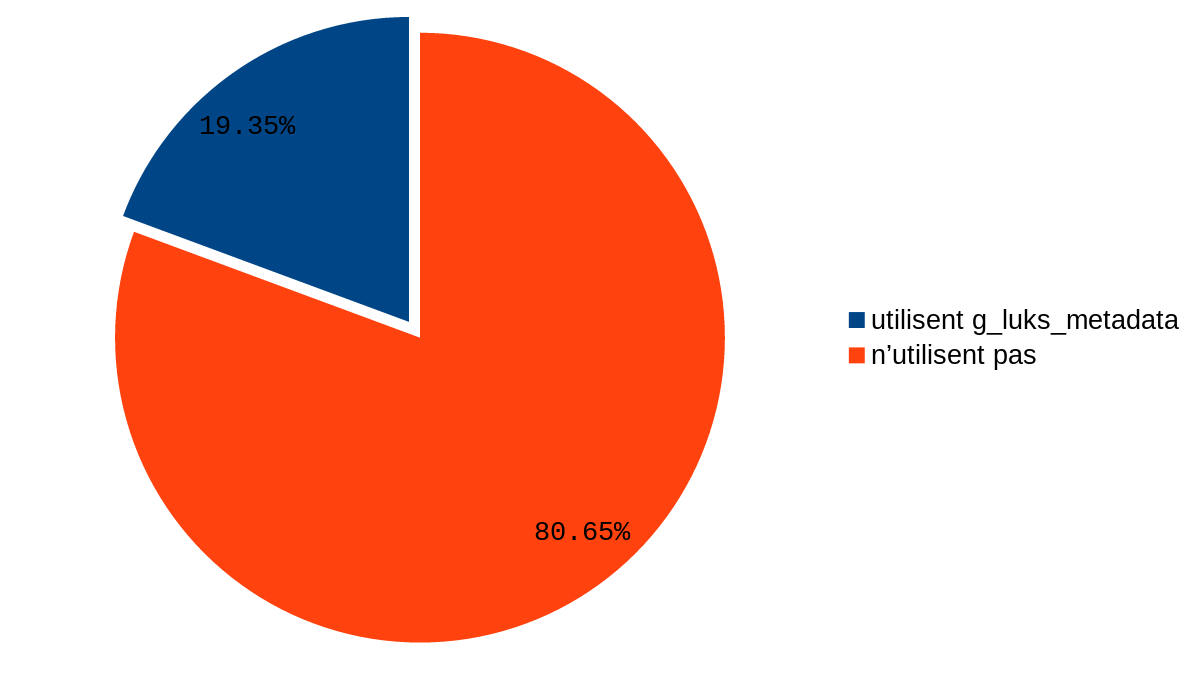
\includegraphics[width=.9\linewidth]{choix_developpement/fonctions_g_luks_metadata.png}
\caption{\label{fig:fonctions_md}Fonctions utilisant les métadonnées}
\end{figure}
\paragraph{}
\begin{figure}[h]
\centering
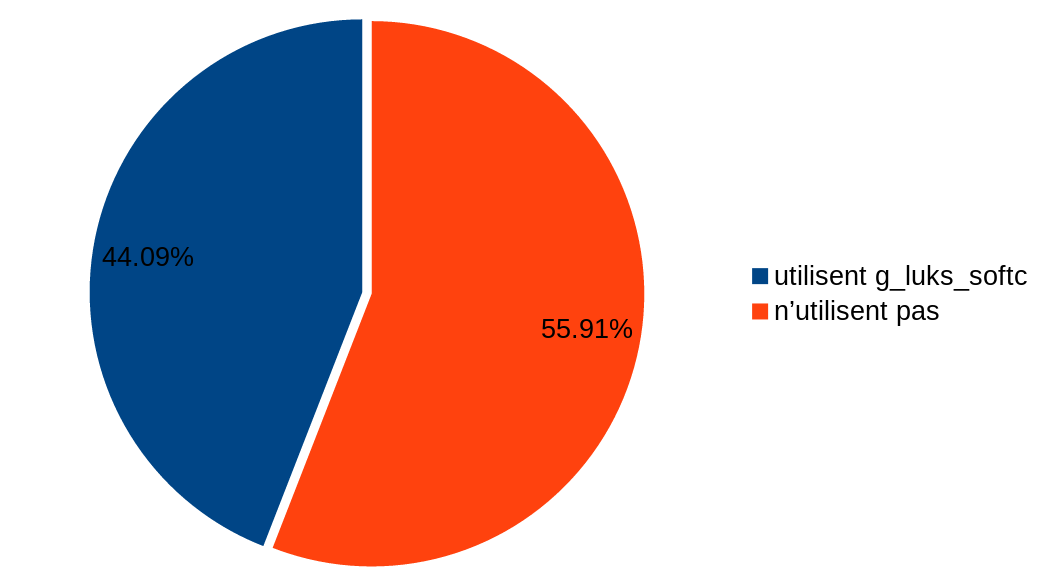
\includegraphics[width=.9\linewidth]{choix_developpement/fonctions_g_luks_softc.png}
\caption{\label{fig:fonctions_sc}Fonctions utilisant la structure \texttt{softc}}
\end{figure}
\paragraph{}
C'est pourquoi, la solution la plus intéressante serait de garder la structure
de \textit{GELI} et d'y mettre les informations de chiffrement. Cela permettra 
notamment d'écrire et/ou de modifier moins de code et donc de limiter les erreurs
et de faciliter la maintenabilité. De plus en choisissant de procéder ainsi, on
peut modifier le code facilement par itérations en le gardant compilable et 
exécutable. On choisit donc de conserver le code de 
GELI le plus possible et de transformer les métadonnées de LUKS en métadonnées 
GELI.

\paragraph{}
En effet bien que les métadonnées stockées sur le disque soient différentes 
entre GELI et LUKS, le chiffrement du disque reste essentiellement identique :
on utilise une clé maître et un algorithme de chiffrement de blocs. Cependant 
comme décrit auparavant, la clé maître dans GELI est dérivée en clés de 
chiffrement. Toutefois, GELI laisse la possibilité à travers des {\em Flags} 
d'utiliser la clé maître comme unique clé de chiffrement.

\paragraph{}
Comme décrit en \ref{ssec:md_usage}, les métadonnées utilisées par l'instance
GEOM sont celles qui sont stockées dans la stucture {\em softc}, à l'exception
de la lecture sur disque des métadonnées et de leur vérification ainsi que le 
changement des métadonnées sur le disque (changement de la phrase de passe et
donc de la clé chiffrée sur le disque).

\paragraph{}
\begin{figure}[h]
\centering
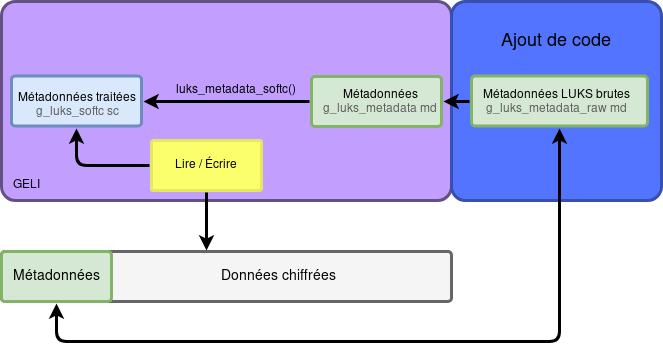
\includegraphics[width=.9\linewidth]{choix_developpement/utilisation_metadonnee_luks.png}
\caption{\label{fig:transformation_md}Transformation des métadonnées}
\end{figure}

\paragraph{}
La transformation des métadonnées LUKS en métadonnées GELI consiste donc à 
remplacer la lecture des métadonnées du disque par GELI par celles de LUKS 
comme illustré par le schéma \ref{fig:transformation_md}. On change donc la 
fonction {\em luks\_metadata\_softc} pour qu'elle utilise les données extraites
de l'en tête LUKS du disque au lieu de celles extraites de l'en tête GELI, donc
respectivement du premier secteur et de quelques secteurs suivant au lieu du 
dernier secteur. On devra également changer la gestion du déchiffrement de la 
clé du disque.


\subsubsection{Déchiffrement de la clé de chiffrement dans le cas de GELI}
Dans le cas de GELI, le code prévoit le déchiffrement de la clé de chiffrement 
dans le noyau, de façon à pouvoir déchiffrer le disque au démarrage (pour 
pouvoir déchiffrer un volume racine chiffré). Plus précisément l'utilitaire en espace
utilisateur envoie au noyau via l'API de GEOM, la phrase de passe dérivée via
l'algorithme PKCS5v2 en prenant SHA512 comme fonction pseudo aléatoire.


\subsubsection{Déchiffrement de la clé de chiffrement dans le cas de LUKS}
\label{sub:dechif_cle}
\paragraph{}
On a donc besoin de déchiffrer la clé de chiffrement stockée dans l'en-tête LUKS.
Pour cela il faut tout d'abord bien comprendre comment est stockée la clé de 
chiffrement sur le disque.

\paragraph{}
La clé de chiffrement est hashée selon l'algorithme spécifié par le champ
{\em hash-spec}, et stockée dans le champ {\em mkdigest} (Master Key Digest).

L'en-tête LUKS permet de stocker la même clé chiffrée avec huits phrases de passe
différentes, dans les huits {\em KeySlot} définis par le standard.
\\
Pour un keyslot, la phrase de passe est dérivée selon l'aglorithme {\em PKCS5v2}
avec comme fonction pseudo aléatoire l'algorithme de hashage spécifié par 
{\em hash-spec}. La clé est ensuite fragmentée via l'algorithme 
{\em anti-forensic splitter} spécifié dans \cite{AFsplitting} qui a pour but de
lutter contre la persistance des informations stockées sur des disques durs
(disques qui utilisent le magnétisme pour stocker les données)
\\
Enfin le résultat de la fragmentation est chiffré selon l'algorithme utilisé 
pour les données du disque (donc précisé par les champs {\em cipher-name} et 
{\em cipher-mode}) avec comme clé le résultat de la dérivation de la phrase de
passe.

\paragraph{}
Une différence avec {\em GELI} est que le nombre d'itérations utilisé pour 
{\em PKCS5v2} est différent pour chaque keyslot alors que pour {\em GELI} c'est
le même pour toutes les phrases de passe.
Dans {\em GELI} la phrase de passe est dérivée en espace utilisateur avant 
d'être envoyée en espace noyau, qui déchiffrera ensuite la clé de chiffrement.
Or si l'on applique le même procédé pour {\em LUKS}, il faut alors dans le cas
où les 8 keyslot sont actifs, envoyer 8 phrases de passe dérivées au noyau.
Il est donc plus simple d'envoyer la phrase de passe directement au noyau, qui
effectuera donc tout les calculs.

\subsubsection{Choix concernant la clé de chiffrement}
\paragraph{}
On a choisi de transformer les métadonnées de {\em LUKS} en métadonnées 
{\em GELI}, cependant on ne peut pas vraiment passer du format {\em LUKS} à 
{\em GELI} pour la clé de chiffrement. En effet, si on voulait écrire la clé 
de chiffrement dans les métadonnées {\em GELI}, il faudrait déchiffrer la clé 
présente sous le format {\em LUKS} puis la rechiffrer sous le format {\em GELI}
pour ensuite la déchiffrer. Ce serait réaliser des opérations en plus, qui ne 
sont pas nécessaires et il faudrait en plus de cela choisir une phrase de passe
pour le rechiffrement de la clé au format {\em GELI}. 

\paragraph{}
La clé de chiffrement étant déjà traitée de façon séparée dans le code de 
{\em GELI}, on choisit de traiter la clé de façon séparée également et donc de 
ne pas la transformer au format {\em GELI}


\subsubsection{Sélection des algorithmes utilisés}
\paragraph{}
Deux données importantes sont nécessaires pour le chiffrement et déchiffrement
de disque: l'algorithme de chiffrement utilisé ainsi que la méthode de
génération du vecteur d'initialisation \textbf{IV}. Dans notre cas, l'algorithme
de chiffrement peut être \textbf{aes-xts}, \textbf{aes-cbc} ou
\textbf{cast5-cbc}. Chacun de ces algorithmes n'accepte pas les même méthodes de
génération de l'\textbf{IV}, qui peut être de type \textit{plain} (32 ou 64) ou
\textit{essiv:sha256}. Bien que le standard proposé par le créateur
d'\textit{essiv} n'interdise pas l'utilisation d'autres algorithmes de hachage
(comme le suggère la syntaxe de la commande), seul \texttt{SHA256} peut être
utilisé avec \textit{essiv} dans \textit{cryptsetup}. Le vecteur
d'initialisation est unique à chaque secteur du volume chiffré. Il doit donc
être recalculé pour chaque secteur. Cela permet de ne pas avoir besoin de
déchiffrer l'intégralité du volume pour accéder à une ressource placée à la fin
des données chiffrées. Cela permet également paralléliser les processus gérant
le chiffrement ou déchiffrement d'un même disque, puisque chaque secteur pourra
être manié indépendamment des autres. Le premier type prend numéro du secteur
concerné codé sur 32 ou 64 bits comme vecteur d'initialisation, tandis que
\textit{essiv:sha256} (pour \textbf{e}ncrypted \textbf{s}ector-\textbf{s}alt
\textbf{i}nitialisation \textbf{v}ector) calcule l'IV à partir d'une combinaison
du numéro de secteur avec le hachage de la clé de chiffrement.
\paragraph{}
\begin{figure}[h]
\centering
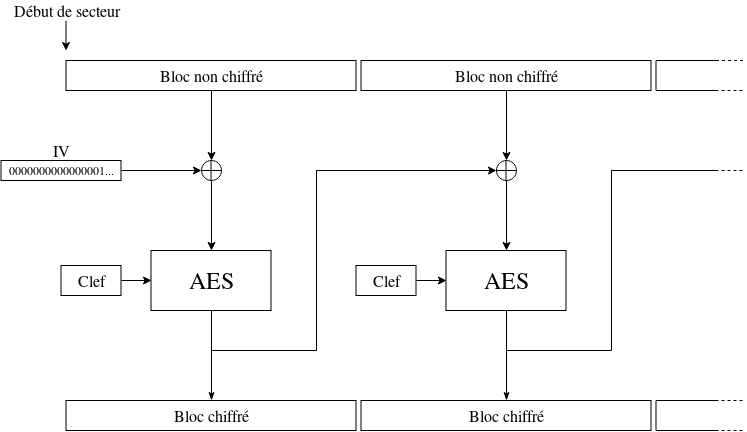
\includegraphics[width=.9\linewidth]{choix_developpement/aes_cbc.png}
\caption{\label{fig:aes_cbc}Chiffrement en AES-CBC}
\end{figure}
\paragraph{}
Dans les métadonnées \textit{LUKS}, deux champs distincts permettent à
\textit{dm-crypt} de connaître l'algorithme de chiffrement utilisé ainsi que la
manière dont le vecteur d'initialisation \texttt{IV} est calculé:
\begin{itemize}
\item \textbf{Cipher name}: nom de l'algorithme de chiffrement utilisé
\item \textbf{Cipher mode}: manière dont le vecteur d'initialisation est généré
\end{itemize}
\paragraph{}
Dans les métadonnées \textit{GELI}, ces deux informations sont confondues dans
le champs \textbf{ealgo} (\textit{encryption algorithm}). La variable est
ensuite enregistrée et utilisée dans la structure \texttt{softc}. Le calcul de
\textbf{IV} quant à lui est géré par la fonction \texttt{g\_eli\_crypto\_ivgen},
qui est en mode \textit{plain64} lorsque l'algorithme \textbf{aes-xts} est
utilisé, et \textit{essiv:sha256} autrement.
\paragraph{}
Par défaut, le type d'\textbf{IV} (le \texttt{cipher mode} dans \textit{LUKS})
calculé par la fonction de \textit{GELI} dépend de l'algorithme de chiffrement
(le \textit{cipher name} dans \textit{LUKS}). Cette y association est codée en
dur:
\begin{itemize}
\item le calcul de l'\textbf{IV} est équivalent au mode \texttt{plain64} de
  \textit{LUKS} lorsque l'algorithme \textbf{AES-XTS} est indiqué
\item le calcul correspond au mode \texttt{essiv:sha256} de \textit{LUKS}
  autrement
\end{itemize}
\paragraph{}
En gardant la fonction \textit{GELI} calculant l'\textbf{IV} telle quelle, la
liste d'algorithmes possibles se restreint aux choix suivants:
\begin{center}
  \begin{tabular}{ | l | l | }
    \hline
    \textbf{Cipher name} & \textbf{Cipher mode}  \\
    \hline
    AES-XTS              & \texttt{plain64}      \\
    AES-CBC              & \texttt{essiv:sha256} \\
    CAST5-CBC            & \texttt{plain}        \\
    \hline
  \end{tabular}
\end{center}
\paragraph{}
Cependant, \textit{LUKS} ne gérant pas l'authentification des données et
\textit{GELI} le faisant, il est possible d'utiliser le champs \texttt{aalgo}
devenu inutile, pour pouvoir stocker le \textit{cipher mode} indépendamment du
\textit{cipher name}. En faisant cela, seule la fonction chargée du calcul de
\textbf{IV} doit être modifiée, mais les structures \texttt{metadata} et
\texttt{softc} héritées de \textit{GELI} restent inchangées.
\paragraph{}
Le nombre de choix possibles se limite maintenant aux associations suivantes:
\begin{center}
  \begin{tabular}{ | l | l | }
    \hline
    \textbf{Cipher name} & \textbf{Cipher mode}  \\
    \hline
    AES-XTS              & \texttt{plain64}      \\
    AES-CBC              & \texttt{plain}        \\
    AES-CBC              & \texttt{essiv:sha256} \\
    CAST5-CBC            & \texttt{plain}        \\
    \hline
  \end{tabular}
\end{center}
\paragraph{}
Cette limite est due à l'implémentation native des algorithmes dans le système,
qui doivent à la fois être présents dans le standard \textit{LUKS} et supportés
par \textit{FreeBSD}.


\subsubsection{Noyau et espace utilisateur}
\paragraph{}
Pour implémenter le support de {\em LUKS} sur {\em FreeBSD}, et donc de nouvelles
fonctions, ainsi que la modification de fonctions existantes de {\em GELI}, il
faut savoir pour chaque fonction si elle est utilisée dans le noyau ou en espace
utilisateur ou encore si elle est utilisée dans les deux cas. En effet, on peut
par exemple citer l'utilisation de la fonction {\em malloc} qui diffère entre
le noyau et l'espace utilisateur, on peut également noter que l'utilisation des
fonctions de chiffrement se fait à travers l'API {\em opencrypto} dans le noyau
et à travers la bibliothèque {\em OpenSSL} en espace utilisateur. 

\paragraph{}
Dans l'outil en espace utilisateur permettant d'intéragir avec le module 
{\em geom\_eli} (dont le fichier source est /sbin/geom/class/eli/geom\_eli.c),
on peut noter les deux inclusions :
\begin{lstlisting}
#include <geom/eli/g_eli.h>
#include <geom/eli/pkcs5v2.h>
\end{lstlisting}

\paragraph{}
Donc les fonctions utilisées directement par l'outil en espace utilisateur sont
celles dont le prototype ou la définition se trouve dans {\em g\_eli.h} et
{\em pkcs5v2.h}. On y trouve les structures correspondant aux métadonnées brutes
comme traitées ({\em g\_eli\_metadata,g\_eli\_softc}) mais aussi les fonctions
pour décoder et encoder les métadonnées et la fonction qui permet de passer de
{\em g\_eli\_metadata} à {\em g\_eli\_softc}. Enfin on y trouve les fonctions 
permettant de chiffrer et déchiffrer la clé maître, avec donc des fonctions
permettant d'effectuer des opérations de chiffrement et déchiffrement.


\paragraph{}
Si l'on s'intéresse aux objets qui sont assemblés pour produire la bibliothèque
geom\_luks.o qui est ensuite installée sur le système, on peut noter la présence
des 4 fichiers suivants :
\begin{itemize}
	\item g\_eli\_crypto.c
	\item g\_eli\_hmac.c
	\item g\_eli\_key.c
	\item pkcs5v2.c
\end{itemize}

\paragraph{}
Le fichier {\em g\_eli\_crypto.c} contient les fonctions permettant de réaliser
du chiffrement et déchiffrement qui sont donc implémentées deux fois (une fois
pour le noyau, une autre pour l'espace utilisateur). Le fichier
{\em g\_eli\_hmac.c} contient quand à lui une implémentation des fonctions
permettant de calculer des HMAC avec l'algorithme SHA512. Une seule implémentation
est présente, elle est compatible entre le noyau et l'espace utilisateur, du fait
que les fonctions et types associés à SHA512 sont les mêmes entre le noyau et
l'espace utilisateur.
Cependant l'API {\em opencrypto} implémente déjà l'algorithme de HMAC avec SHA512.
La réimplémentation de l'algorithme permettant le calcul d'un HMAC peut très
probablement s'expliquer du fait qu'elle permet d'avoir un code plus restreint,
et donc plus facilement maintenable.

Le fichier {\em g\_eli\_key.c} contient quant à lui les fonctions permettant de
chiffrer, déchiffrer et vérifier la clé maître, en utilisant les fonctions de
{\em g\_eli\_crypto.c}.

Enfin le fichier {\em pkcs5v2.c} contient les fonctions permettant le calcul
d'une clé dérivée à partir d'une phrase de passe à travers le standard
{\em PKCS5v2}, en utilisant les fonctions de {\em g\_eli\_hmac.c}.

\paragraph{}
Dans l'implémentation du module {\em geom\_luks} on doit pouvoir être capable
d'utiliser l'algorithme {\em PKCS5v2} avec SHA512 comme dans {\em GELI} mais
aussi avec {\em SHA1,SHA256,RIPEMD160}. Cela peut-être très simple en utilisant
l'API {\em opencrypto} qui prévoit déjà leur utilisation, cependant conserver
le modèle de {\em GELI} imposerait l'implémentation de l'algorithme HMAC utilisant
les autres algorithmes de hashage, et dupliquerait donc du code. Il faudrait
donc factoriser ou savoir si l'utilisation de {\em PKCS5v2} et du {\em HMAC}
en espace utilisateur est indispensable. De plus les noms de fonctions qui
correspondent à l'algorithme SHA1 diffèrent entre le noyau et l'espace
utilisateur, il faudrait donc dupliquer le code ou factoriser en modifiant
légèrement les sources de SHA1 dans le noyau (ajouter des noms possibles pour
les différentes fonctions).

\paragraph{}
Le fichier {\em geom\_eli.c} révèle que ces fonctions sont utilisées pour réaliser
des opérations sur la phrase de passe, qui sont donc réalisées uniquement ou
en partie en espace utilisateur.

\paragraph{}
Pour simplifier l'implémentation, on choisi d'implémenter toutes les opérations
dans le noyau pour les raisons évoquées ci-dessus, et pour permettre un 
déchiffrement plus simple de la clé maître comme évoqué en \ref{sub:dechif_cle}.
\paragraph{}
On implémente donc les différentes fonctions pour déchiffrer la clé maître à
partir de la phrase de passe. Ce qui nous permet donc d'arriver à la création
du disque déchiffré, après avoir traduit correctement les métadonnées de
{\em GELI} en métadonnées {\em LUKS}, on obtient donc un fonctionnement
comme décrit par le schéma \ref{fig:fonctionnement}


\begin{figure}[h]
\centering
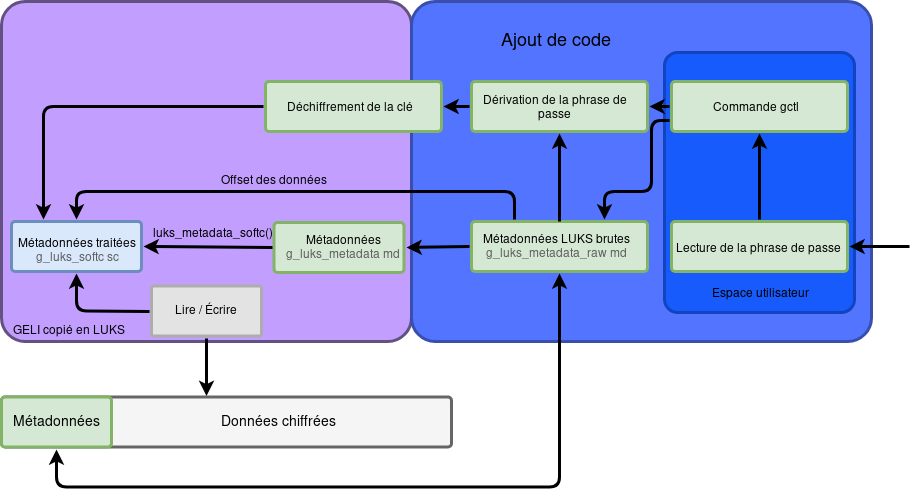
\includegraphics[width=\linewidth]{choix_developpement/utilisation_metadonnee_luks_2.png}
\caption{\label{fig:fonctionnement}Fonctionnement de GEOM LUKS}
\end{figure}

\subsubsection{Champ drapeaux: \texttt{md\_flags}}
\paragraph{}
Certains paramètres, indispensables à \textit{GELI} pour manipuler des disques
chiffrés, n'ont pas d'équivalents dans les métadonnées \textit{LUKS} et ne
peuvent donc pas être traduits d'un standard à l'autre. Il peuvent correspondre
par exemple à l'authentification des données, prise en charge par \textit{GELI}
mais pas \textit{LUKS}. D'autres champs décrivant comment sont chiffrées les
données, en dehors des algorithmes utilisés.
\paragraph{}
Ce champ est présent dans les structures \texttt{metadata} et \texttt{softc} de
\textit{GELI}. Il précise les différentes options possibles pour le chiffrement
de disques et garanti ainsi la compatibilité entre les différentes versions de
\textit{GELI}. La version actuelle comprend 16 drapeaux: \\
\\
\begin{tabularx}{\linewidth}{ | l | X | }
  \hline
  \textbf{Drapeau}                            & \textbf{Description} \\
  \hline
  \texttt{G\_ELI\_FLAG\_ONETIME}             & Utiliser des clés aléatoires et
  uniques \\
  \texttt{G\_ELI\_FLAG\_BOOT}                & Demander la phrase de
  chiffrement au noyau, avant de monter \texttt{root} \\
  \texttt{G\_ELI\_FLAG\_WO\_DETACH}          & Détacher le volume à la dernière
  fermeture, si nous étions ouverts à l'écriture \\
  \texttt{G\_ELI\_FLAG\_RW\_DETACH}          & Détacher le volume à la dernière
  fermeture \\
  \texttt{G\_ELI\_FLAG\_AUTH}                & Proposer l'authentification des
  données \\
  \texttt{G\_ELI\_FLAG\_RO}                  & Le volume est en lecture seule,
  toute tentative d'écriture serait refusée \\
  \texttt{G\_ELI\_FLAG\_NODELETE}            & Ne pas ignorer les requêtes
  \texttt{BIO\_DELETE} \\
  \texttt{G\_ELI\_FLAG\_GELIBOOT}           & Cette version de \textit{GELI}
  supporte \textit{GELIBoot} \\
  \texttt{G\_ELI\_FLAG\_GELIDISPLAYPASS}    & Masquer la longueur de la phrase
  de chiffrement dans \textit{GELIboot} \\
  \texttt{G\_ELI\_FLAG\_WOPEN}               & Le volume autorise l'écriture \\
  \texttt{G\_ELI\_FLAG\_DESTROY}             & Détruire le volume \\
  \texttt{G\_ELI\_FLAG\_NATIVE\_BYTE\_ORDER} & Le volume utilise l'ordre natif
  d'octets pour la générer du vecteur d'initialisation \\
  \texttt{G\_ELI\_FLAG\_SINGLE\_KEY}         & Le volume utilise une seule clé
  de chiffrement \\
  \texttt{G\_ELI\_FLAG\_SUSPEND}             & Dispositif suspendu \\
  \texttt{G\_ELI\_FLAG\_FIRST\_KEY}          & Le volume utilise la première
  clé de chiffrement \\
  \texttt{G\_ELI\_FLAG\_ENC\_IVKEY}          & Le volume utilise l'IV-Key pour
  générer la clé de chiffrement \\
  \hline
\end{tabularx}
\paragraph{\texttt{G\_ELI\_FLAG\_BOOT}}
Ce drapeau permet au système de démarrer même si la partition \texttt{root} est
chiffrée. Il serait donc possible de l'utiliser pour la chiffrer avec
\textit{LUKS} (si les fonctions permettant le déchiffrement d'un volume
\textit{LUKS} existent), et doit donc être activé dans ce cas précis.
\paragraph{\texttt{G\_ELI\_FLAG\_AUTH}}
\textit{LUKS} ne supportant pas l'authentification des données, ce drapeau est
désactivé pour ignorer les fonctions et les champs normalement utilisés par
\textit{GELI} pour réaliser cette action. Ce drapeau doit être désactivé.
\paragraph{\texttt{G\_ELI\_FLAG\_SINGLE\_KEY}}
Dans la plupart des versions de \textit{GELI}, la clé maître est dérivée pour
chiffrer chaque secteur. Cependant, \textit{LUKS} ne la dérive pas et utilise la
même clé pour chiffrer tout le volume. Ce drapeau doit alors être activé, car
il permet d'indiquer aux fonctions de \textit{GELI} de ne pas dériver la clé
pour chaque secteur, et ainsi fonctionner comme \textit{LUKS} dans ce cas
précis.

\subsubsection{Nombre de clés actives: \texttt{md\_keys}}
Dans les métadonnées \textit{GELI}, une variable correspond au nombre de clés
permettant le déchiffrement de la clé maître, et donc du volume chiffré. Dans
\textit{LUKS}, on peut savoir si l'emplacement d'une clé est actif ou non; il y
a en tout 8 emplacements. Une boucle permet alors de parcourir tous les
emplacements et savoir s'ils sont actifs ou non, et ainsi de connaître le nombre
de phrases secrètes à indiquer dans les métadonnées.
% LocalWords:  LUKS GELI GEOM keys md KEY FLAG AUTH root BOOT l'IV-Key IVKEY
% LocalWords:  ENC FIRST ORDER BYTE DESTROY WOPEN GELIboot GLUKSDISPLAYPASS
% LocalWords:  GELIBoot GLUKSBOOT

\subsubsection{Création du disque déchiffré}
Avec {\em GEOM} l'API noyau de FreeBSD pour gérer les disques, lorsque l'on
créé un disque à partir d'un autre, la structure comprend notamment, la taille
du disque, la taille d'un secteur. Pour calculer la taille du disque, il faut
soustraire de la taille du de la partition complète, la taille de l'en-tête. 
Avec les métadonnées de {\em LUKS} on a directement le champ {\em payloadoffset}
qui permet de connaître le nombre de secteurs qu'occupent l'en-tête. Comme sous
{\em GELI} les métadonnées sont à la fin du disque, il n'y a pas de
transformation à faire sur le numéro de secteur lors de lectures ou écritures.
Cependant avec {\em LUKS}, comme les métadonnées sont au début, il faut prévoir
ce décalage. {\em GELI} ne réalisant pas cette opération, on rajoute
à la structure {\em softc} un champ {\em sc\_offset} que l'on utilise dans les
fonctions de lecture et écriture sur disque.


\section{Gestion des disques}

\subsubsection{Différences entre \textit{device-mapper} de Linux et
  \textit{GEOM} de FreeBSD}
\paragraph{}
La principale différence entre ces deux systèmes se situe au niveau de
l'emplacement des métadonnées.
\paragraph{}
Dans un système Linux, \textit{device-mapper} laisse à l'outil qui va l'utiliser
(comme \textit{cryptsetup} qui passe par \textit{dm-crypt, une classe
  \textit{device-mapper}}) la gestion totale des données sur le volume qui lui
est présenté. Côté FreeBSD en revanche, un outil et une classe \texttt{GEOM}
doit passer par les fonctions de base de \textit{GEOM}.

\subsubsection{Application des fonctions \textit{GELI} à un disque chiffré \textit{LUKS}}
\paragraph{}
Dans notre cas, on appelle l'outil l'ensemble des commandes qui entrées par
l'utilisateur afin de gérer le disque chiffré. Par défaut, l'outil \textit{GELI}
appelle une fonction de \textit{GEOM} qui va chercher les métadonnées sur le
volume pour les enregistrer dans une structure passée en paramètre. Cependant,
cette fonction ne laisse pas le choix de leur emplacement et cherche à les lire
directement à la fin du volume en fonction de sa taille et de la taille de la
structure. Pour développer notre outil \textit{GLUKS} avec un fonctionnement
semblable à celui de \textit{GELI}, il est nécessaire d'écrire une fonction
similaire ayant pour vocation d'aller chercher ces métadonnées au début du
disque plutôt qu'à la fin.
\paragraph{}
La classe \textit{GEOM} est l'ensemble des fonctions permettant la gestion de
disque côté noyau. Pour la lecture et l'écriture des métadonnées, les fonctions
de la classe \textit{GELI} ne dépendent pas de fonctions \textit{GEOM} de base.
Elles cherchent toujours l'emplacement des métadonnées à la fin du volume mais
calcule cette fois-ci elle-même l'\texttt{offset} à partir duquel elles se
trouvent. Afin d'adapter la classe \textit{GELI} à notre classe \textit{GLUKS},
il est nécessaire de mettre cet \texttt{offset} à \texttt{0} à chaque fois qu'on
aura à lire ou écrire des données sur le disque, qu'il s'agisse de métadonnées
ou de données utiles. 

\section{Passage de l'espace utilisateur au noyau}
Nous avions donc besoin d'envoyer au noyau la phrase de passe, pour cela il a
fallu comprendre comment l'utilitaire {\em geom\_eli} passait des commandes et
des valeurs au module noyau {\em geli}. Le code de {\em GELI} a donc encore une
fois servi d'exemple.

\subsection{GEOM}
\paragraph{}
L'API {\em GEOM} s'utilise donc dans le noyau comme nous l'avons vu mais
également sous la forme d'une bibliothèque que l'on utilise en espace
utilisateur permettant de générer automatiquement la sortie de la commande 
{\em help} pour l'utilitaire par exemple, et bien sur les fonctions permettant
de changer de contexte en envoyant à la classe GEOM associée des commandes ainsi
que des valeurs.

\paragraph{}
Pour générer la sortie de la commande help, ainsi que pour permettre à GEOM de
vérifier la cohérence des commandes envoyées, la structure {\em g\_command} est
déclarée dans le code source de l'utilitaire, le développeur n'a ensuite qu'à 
utiliser les commandes conformément à la structure sans avoir besoin de
l'utiliser. La structure est utilisée par la bibliothèque pour générér
automatiquement la commande help et vérifier la cohérence des commandes passées
au noyau. D'ailleurs concernant commandes,
l'utilitaire sert en fait à remplir la structure {\em gctl\_req} à partir des
entrées utilisateurs, puis de l'envoyer au noyau via la fonction
{\em gctl\_issue}. Du côté noyau, une fonction permet selon le type de commande
d'appeler la fonction adéquate avec en argument la structure gctl\_req reçue,
dont les variables sont utilisée pour accomplir la tâche demandée.

\section{Confidentialité}
\paragraph{}
Comme nous l'avons constaté en utilisant le code de {\em GELI}, les variables
qui contiennent des données qui pourraient porter atteinte à la confidentialité
sont écrasée avec des zéros dès qu'elles ne sont plus utiles, y compris avant
le retour de la fonction. Cela permet de rendre les attaques sur le module
noyau ou la mémoire vive plus complexe, pour obtenir la clé de déchiffrement ou
la phrase de passe du disque. En effet, on utilise l'instruction {\em bzero}
sur les variables sensibles (la clé de chiffrement, la phrase de passe, la
phrase de passe dérivée, etc.) dès que l'on peut. Ainsi une fois le disque
monté, uniquement la clé de chiffrement est présente en mémoire pour pouvoir
lire et écrire sur le disque chiffré.
